\section[Paper III: Neural network analysis of sleep stages enables efficient diagnosis of narcolepsy]{Paper III: Neural network analysis of sleep stages enables efficient diagnosis of narcolepsy%
    \sectionmark{Stephansen \& Olesen et al., 2018}}\label{sec:paperiii-narcolepsy}
\sectionmark{Stephansen \& Olesen et al., 2018}

% \protect\graffito{Sleep stage classification using neural networks is described in~\cref{chap:sleep-stage-classification}}
\begin{tcolorbox}[colframe=white]
\paragraph{Abstract:} Analysis of sleep for the diagnosis of sleep disorders such as \ac{NT1} currently requires visual inspection of polysomnography records by trained scoring technicians. 
Here, we used neural networks in approximately \num{3000} normal and abnormal sleep recordings to automate sleep stage scoring, producing a hypnodensity graph---a probability distribution conveying more information than classical hypnograms. 
% Accuracy of sleep stage scoring was validated in 70 subjects assessed by six scorers. 
% The best model performed better than any individual scorer (87\% versus consensus). 
% It also reliably scores sleep down to \SI{5}{\second} instead of \SI{30}{\second} scoring epochs.
A \ac{NT1} marker based on unusual sleep stage overlaps achieved a specificity of 96\% and a sensitivity of 91\%, validated in independent datasets. 
Addition of \hla typing increased specificity to 99\%. 
Our method can reduce time spent in sleep clinics and automates \ac{NT1} diagnosis. 
It also opens the possibility of diagnosing \ac{NT1} using home sleep studies.
\end{tcolorbox}

\subsection{Methods}

The following sections describe the narcolepsy model aspects in detail from initial hypnodensity computation, to feature engineering, and finally data modeling using \ac{GP} classification algorithms.
The main outcome of this approach is to be able to classify a hypnodensity representation of a \ac{PSG} as either being positive or negative for \ac{NT1}.

\subsubsection{Data descriptions}

\paragraph{Patient-based Austrian Hypersomnia Cohort}
Patients in this cohort were examined at the Innsbruck Medical University in Austria as described in~\citeauthor{Frauscher2013}~\cite{Frauscher2013}.
The AHC contains 118 \acp{PSG} in 86 high pretest probability patients for narcolepsy (see~\cref{tab:sleep-stages:paper-iii:table-s01} for details).
42 patients (81 studies) are clear T1N with cataplexy cases, with all but 3 having a positive MSLT (these three subjects had a mean sleep latency (MSL)>8 minutes but multiple SOREMPs).
The rest of the sample has idiopathic hypersomnia and type 2 narcolepsy.
Four patients have an AHI>15/hour and 25 had a PLMI>15/hour.
Almost all subjects had two sleep recordings performed, which were kept together such that no two recordings from the same subject were split between training and testing partitions.

% \begin{landscape}
\begin{table}[tb]
\begin{adjustwidth*}{}{-\marginparwidth-\marginparsep}
\small
\centering
\begin{threeparttable}  
\caption[\acs{STAGES} cohorts]{Description of the various cohorts included in this study and how they were used.}
\label{tab:classification-sleep-disorders:paper-iii:table-s01}
\begin{tabular}{@{}lccccccccc@{}}
    \toprule
    \textbf{Cohort}         & \textbf{Age}, years        & \textbf{BMI}, \si{\kilo\gram\per\meter\squared}        & \textbf{Sex}, \%       & \textbf{Train}  & \textbf{Test}              & \textbf{Replication}            & \textbf{\acs{NT1}}, \% & \textbf{H}, \% \\ \midrule
    \acs{WSC}            & 59.7 $ \pm $ 8.4  & 31.6 $ \pm $ 7.1  & 53.1      & 170                  & 116          & None        & 0        & 0 \\
    \acs{SSC}            & 45.4 $ \pm $ 13.8 & 23.9 $ \pm $ 6.5  & 59.4      & 139                  & 112          & None        & 11.6     & 1.8 \\
    \acs{KHC}            & 29.1 $ \pm $ 13.2 & 24.1 $ \pm $ 4.3  & 58.6      & 87                   & 71           & None        & 45.8     & 54.2 \\
    AHC            & 34.5 $ \pm $ 13.8 & 25.9 $ \pm $ 4.9  & 54        & 42 (76)         & 44 (84) & None        & 52.3     & 47.7 \\
    JCTS           & 53.2 $ \pm $ 9.8  & 31.0 $ \pm $ 4.4  & 57.1      & 7                    & None         & None        & 100      & 0 \\
    IHC            & 33.7 $ \pm $ 17.6 & -           & 56.7      & 87                   & 61           & None        & 47.3     & 50 \\
    DHC            & 33.4 $ \pm $ 14.8 & 24.8 $ \pm $ 4.9  & 50        & 79                   & None         & None        & 26.6     & 48.1 \\
    FHC            & 28.8 $ \pm $ 15.2 & 24.4 $ \pm $ 8.1  & 59        & None                 & None         & 122         & 51.6     & 18 \\
    CNC            & 28.5 $ \pm $ 16.9 & 23.2 $ \pm $ 11.5 & 51.3      & None                 & None         & 199         & 34.2     & 0 \\ \midrule
    Total subjects & & & & 611                  & 404          & 321         &          & \\
    Total \acp{PSG} & & & & 645                  & 444          & 321         &          & \\ \bottomrule% \multicolumn{4}{l}{Total subjects} & 611                  & 404          & 321         &          & \\
    % \multicolumn{4}{l}{Total \acp{PSG}} & 645                  & 444          & 321         &          & \\ \bottomrule
\end{tabular}
\begin{tablenotes}
\footnotesize
\item %
\describe{WSC}; %
\describe{SSC}; %
\describe{KHC}; %
\describe{AHC}; %
\describe{JCTS}; %
\describe{IHC}; %
\describe{DHC}; %
\describe{FHC}; %
\describe{CNC}; %
\describe{NT1}; %
H, unspecific hypersomnia (\ac{NT2} and idiopathic hypersomnia).
\end{tablenotes}
\end{threeparttable}
\end{adjustwidth*}
\end{table}
% \end{landscape}

\paragraph{The Jazz Clinical Trial Sample}
This sample includes seven baseline sleep \acp{PSG} from five sites taken from a clinical trial study of sodium oxybate in narcolepsy (SXB15 with 45 sites in Canada, USA, and Switzerland) conducted by Orphan Medical, now named Jazz Pharmaceuticals.
The few patients included are those with clear and frequent cataplexy (a requirement of the trial) that had no stimulant or antidepressant treatment at baseline~\cite{InternationalXyremStudyGroup2005}.
All 7 subjects in this sample were used exclusively for training the narcolepsy biomarker algorithm.

\paragraph{Patient-based Italian Hypersomnia Cohort}
Patients in this high pretest probability cohort (see~\cref{tab:sleep-stages:paper-iii:table-s01} for demographics) were examined at the IRCCS, Istituto delle Scienze Neurologiche ASL di Bologna in Italy as described in~\citeauthor{Pizza2015}~\cite{Pizza2015}.
The IHC contains 70 \ntI patients (\SI{58}{\percent} male, \plusminus{29.5}{1.9} years old), with either documented low CSF hypocretin levels (59 cases, all but 2 HLA DQB1*06:02 positive), or clear cataplexy, positive MSLTs and HLA positivity (11 subjects).
As non-\ntI cases with unexplained daytime somnolence, the cohort includes 77 other patients: 19 with idiopathic hypersomnia, 7 with type 2 narcolepsy and normal CSF hypocretin-1, 48 with a subjective complaint of excessive daytime sleepiness not confirmed by MSLT, and 3 with secondary hypersomnia.
Subjects in this cohort were used for training (n=87) and testing (n=61) the narcolepsy biomarker algorithm. 

\paragraph{Patient-based Danish Hypersomnia Cohort}
Patients in this cohort were examined at the Rigshospitalet, Glostrup, Denmark as described in~\citeauthor{Christensen2017}~\cite{Christensen2017}.
The DHC contains 79 \acp{PSG} in controls and patients (see~\cref{tab:sleep-stages:paper-iii:table-s01} for details).
Based on \ac{PSG}, multiple sleep latency test and cerebrospinal fluid hypocretin-1 measures, the cohort includes healthy controls (19 subjects), patients with other sleep disorders and excessive daytime sleepiness (20 patients with CSF hypocretin-1 $\geq$ 110 pg/ml), narcolepsy type 2 (22 patients with CSF hypocretin-1 $\geq$ 110 pg/ml), and T1N (28 patients with CSF hypocretin 1 $\leq$ 110 pg/ml).
All 79 subjects in this cohort were used exclusively for training the narcolepsy biomarker algorithm.

\paragraph{Patient-based French Hypersomnia Cohort}
This cohort consists of 122 individual \acp{PSG} recorded at the Sleep-Wake Disorders Center, Department of Neurology, Gui-de-Chauliac Hospital, CHU Montpellier, France (see~\cref{tab:sleep-stages:paper-iii:table-s01} for demographics).
The FHC contains 63 subjects with T1N (all but two tested with CSF hypocretin-1 $\leq$ 110 pg/ml, five below 18 years old, 55 tested for HLA, all positive for HLA DQB1*06:02) and 22 narcolepsy type 2 (19 with CSF hypocretin-1 > 200 pg/ml, and three subjects with CSF hypocretin-1 between 110 and 200 pg/ml, three HLA positive).
The remaining 36 subjects are controls (15 tested for HLA, two with DQB1*06:02) without other symptoms of hypersomnia.
The FHC was used as data for the replication study of the narcolepsy biomarker algorithm.

\paragraph{Patient-based Chinese Narcolepsy Cohort}
This cohort contains 199 individual \acp{PSG} recorded (see~\cref{tab:sleep-stages:paper-iii:table-s01} for demographics).
The CNC contains 67 subjects diagnosed with T1N exhibiting clear-cut cataplexy (55 tested HLA DQB1*06:02 positive), while the remaining 132 subjects are randomly selected population controls (15 HLA DQB1*06:02 positive, 34 HLA negative, remaining unknown)~\cite{Andlauer2012}.
Together with the FHC, the CNC was used as data for the replication study of the narcolepsy biomarker algorithm.

\subsubsection{Model overview}

\begin{figure}
    % \centering
    \begin{adjustwidth*}{}{-\marginparwidth-\marginparsep}
        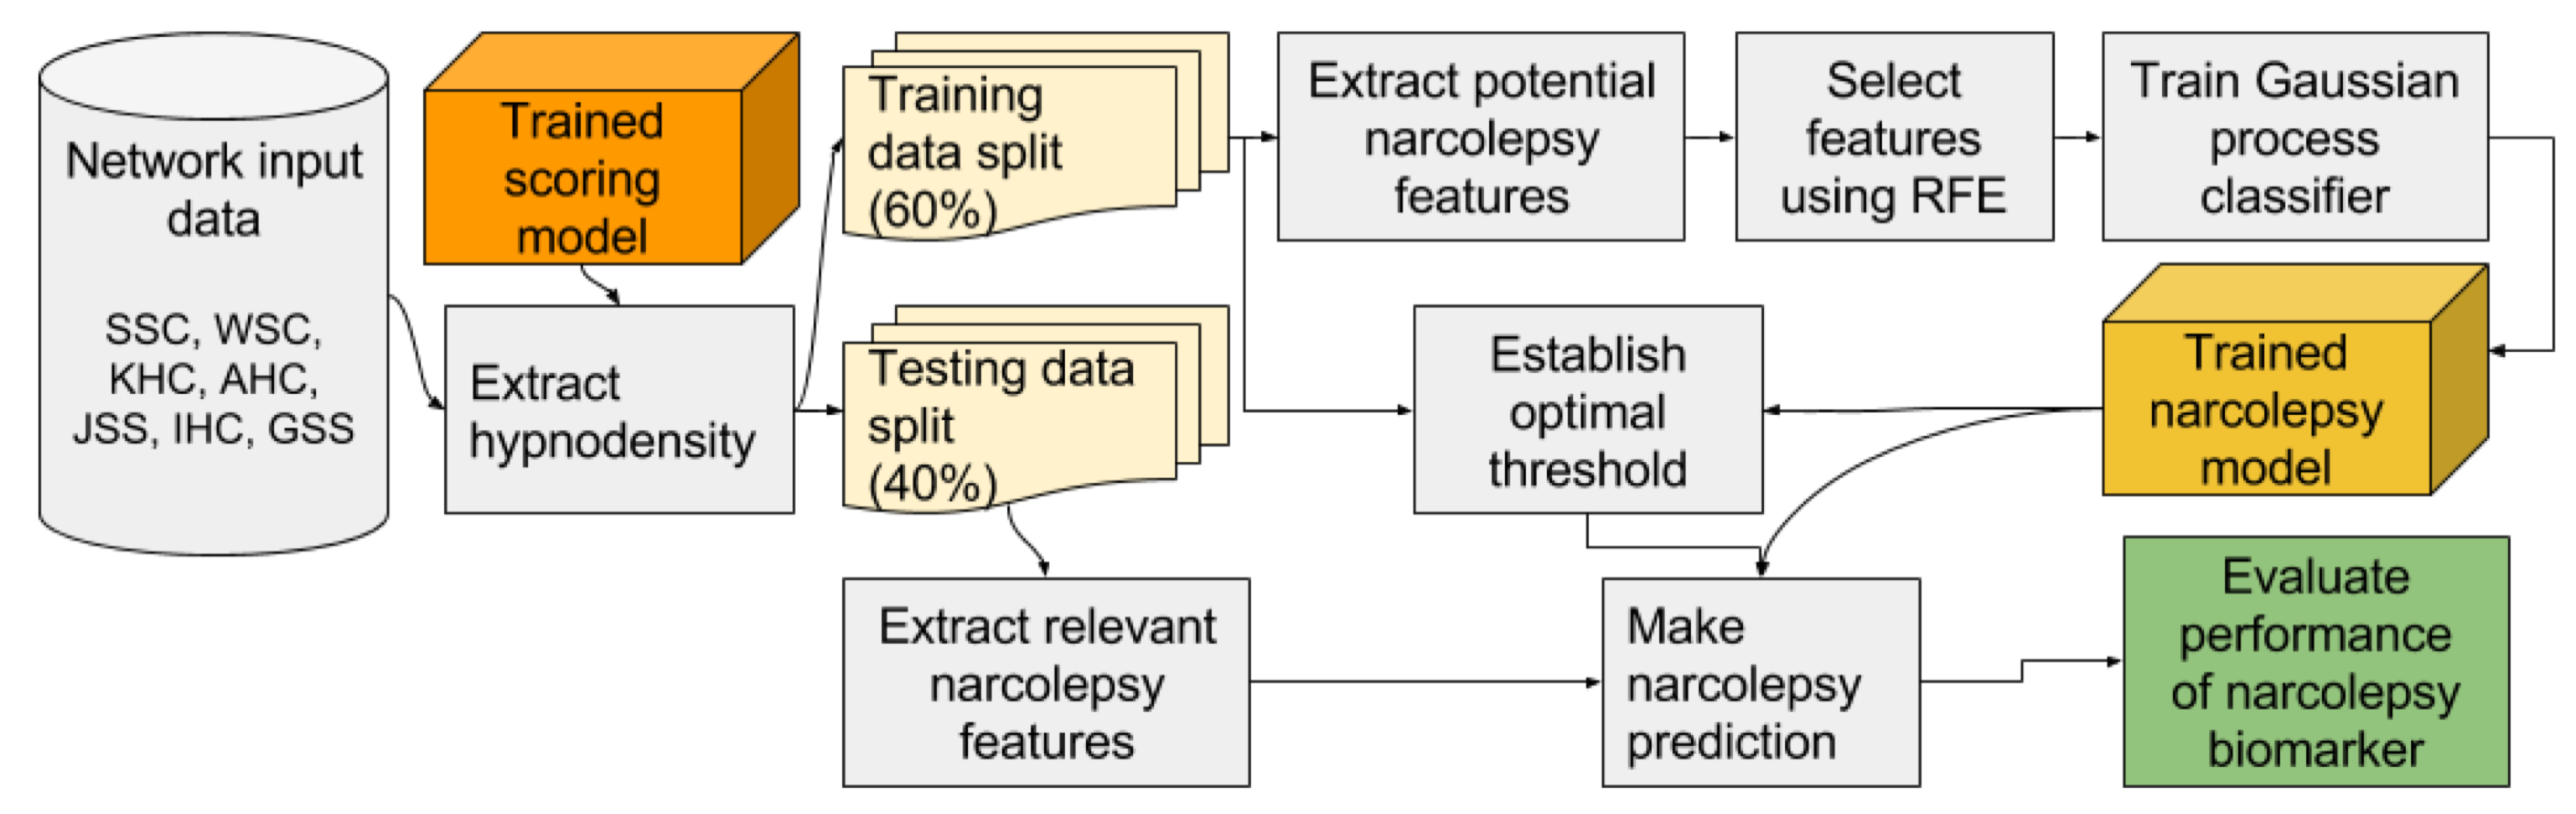
\includegraphics[width=\textwidth+\marginparwidth+\marginparsep]{figures/paper-iii/Figure_5c.png}
        \caption[Narcolepsy detector algorithm design]{Narcolepsy detector algorithm design. Hypnodensities are extracted from data, as described in~\cref{sec:paperiii}. 
        These data are separated into a training (\SI{60}{\percent}) and a testing (\SI{40}{\percent}) split. 
        From the training split, 481 potentially relevant features described in~\cref{tab:sleep-disorders:paper-iii:table-s10} are extracted from each hypnodensity. 
        The prominent features are selected using a \ac{RFE} algorithm, and the narcolepsy detection model is trained using a \ac{GP} model.
        The performance of the \ac{GP} narcolepsy detection  model is evaluated using the selected features computed on the test data.}
        \label{fig:paperiii-figure5c}
    \end{adjustwidth*}
\end{figure}

The general pipeline for training and testing the narcolepsy model is shown in~\cref{fig:paperiii-figure5c}.
The input data sources from the cohorts described in~\cref{tab:classification-sleep-disorders:paper-iii:table-s01} are shown on the left side.
The \acp{PSG} from these cohorts are extracted and subjected to the sleep stage scoring model described in~\cref{sec:paperiii} resulting in a hypnodensity\graffito{The hypnodensity is further described in~\cref{sec:paperiii}, but is essentially a probability distribution over sleep stages.} representation for each \ac{PSG}.

The hypnodensity data are split into training and testing subsets in a \SI{60}{\percent}/\SI{40}{\percent} ratio.
The training data are used for building the \ac{GP} narcolepsy model with a subset of features determined using a feature reduction agorithm.
Cross-validation was employed to determine the optimal classification threshold, and the performance of the classifier was determined on the held-out testing data.

\subsubsection{Feature extraction for \ac{NT1}}

The following sections describe the features computed for each hypnodensity representation.
Overall, the features fall into two categories:
\begin{enumerate*}[label={(\roman*)}]
\item features based on the dynamics between various stage combinations; and,
\item features based on reported findings in the literature.
\end{enumerate*}

\paragraph{Hypnodensity-derived features}
To quantify narcolepsy-like behavior for a single recording \textit{i}, features were generated based on a proto-feature derived from \textit{k}-combinations of $\mathcal{S} = \lbrace \wake, \rem, \nI, \nII, \nIII \rbrace$. 
For the \textit{n}th \num{5}, \num{15} or \SI{30}{\second} segment in recording \textit{i}, a single \textit{k}-combination is selected from the set of all \textit{k}-combinations, and the proto-feature is then calculated as the sum of the pair-wise products of the elements in the single \textit{k}-combination, such that
\begin{equation}
    \func{\boldsymbol{\Phi}^{(i)}_{n}}{\mathcal{S}_{k}} = \sum_{\zeta \in \lbrack \mathcal{S}_{k} \rbrack^2} \prod_{s \in \zeta}{\func{p}{ s \mid \mathbf{x}_{n}^{(i)} }}, \quad p \in \lbrack 0,1 \rbrack,
\end{equation}
where $\boldsymbol{\Phi}^{(i)}_{n}$ is the proto-feature for the \textit{n}th segment in recording \textit{i}, $\zeta \in \lbrack \mathcal{S}_{k} \rbrack^2$ is a 2-tuple, or pair-wise combination, in the set of all pair-wise combinations in the \textit{k}-combination of $\mathcal{S}$, and $s$ is a single element, or sleep stage, in $\zeta$.
For $k \in \llbracket 5 \rrbracket$, there are 31 different $\mathcal{S}_k$, e.g. $\lbrace \wake, \rem \rbrace, \lbrace \nI, \nII, \nIII \rbrace$.
The predicted probability of a 5, 15 or \SI{30}{\second} epoch belonging to a certain class in $\mathcal{S}$ given the data $\mathbf{x}^{(i)}_n$ is given by \( \func{p}{s \mid \mathbf{x}_{n}^{(i)} } \).
For every value of \textit{k}, 15 features based on the mean, derivative, entropy and cumulative sum were extracted as shown in~\cref{tab:sleep-disorders:paper-iii:table-s10}.

\begin{table}[t]
\begin{adjustwidth*}{}{}
\small
\renewcommand{\arraystretch}{1.2}
\begin{threeparttable}
    \caption[Description of narcolepsy features]{Description of each feature, how it is calculated, and how it is numerated.}
    \label{tab:sleep-disorders:paper-iii:table-s10}
    \begin{tabular}{@{}llc@{}} \toprule
        \textbf{\#} & \textbf{Description} & \textbf{Formula} \\ \midrule
        \num{1} & General prevalence of a value & \( \func{\log}{\frac{1}{N} \sum_{n=1}^{N}{\func{\boldsymbol{\Phi}_{n}}{\mathcal{S}_{k}}}} \) \\
        \num{2} & Highest achieved value & \( \func{-\log}{1 - \max \func{\boldsymbol{\Phi}_{n}}{\mathcal{S}_{k}}} \) \\
        \num{3} & Average fluctuations in value & \( \func{\log}{ \frac{1}{N} \sum_{n=1}^{N} \left| \frac{ \mathrm{d} \func{\boldsymbol{\Phi}_{n}}{\mathcal{S}_{k}} }{ \mathrm{d} n } \right| } \) \\
        \num{4} & Log of Shannon entropy & \( \func{\log}{ \frac{-\sum_{i} s_{i}^{2} \log s_{i}^{2}}{N} } \) \\
        \numrange[range-phrase = --]{5}{8} & Time until \textit{p} times max. value & \( \func{\log}{ \func{\mathrm{first}_{p}}{ \frac{ \func{\mathrm{cum \, sum}}{ \func{\boldsymbol{\Phi}}{\mathcal{S}_{k}} }}{ \func{\mathrm{sum}}{ \func{\boldsymbol{\Phi}}{\mathcal{S}_{k}} } } } \times 30} \) \\
        \num{9} & Weighted maximum & \( \sqrt{\max \func{\boldsymbol{\Phi}}{\mathcal{S}_{k}} \times \func{\bar{ \boldsymbol{\Phi}}}{\mathcal{S}_{k}} } \) \\
        \num{10} & Weighted average fluctuation & \( \parentheses*{ \frac{1}{N} \sum_{n=1}^{N} \left| \frac{ \mathrm{d} \func{\boldsymbol{\Phi}_{n}}{\mathcal{S}_{k}} }{ \mathrm{d} n } \right| } \times \func{\bar{ \boldsymbol{\Phi}}}{\mathcal{S}_{k}} \) \\
        \num{11} & Weighted Shannon entropy & \( \func{\log}{ \frac{-\sum_{i} s_{i}^{2} \log s_{i}^{2}}{N} \times \func{\bar{ \boldsymbol{\Phi}}}{\mathcal{S}_{k}} } \) \\
        \numrange[range-phrase = --]{12}{15} & Weighted time until \textit{p} max value & \( \sqrt{ \func{\log}{ \func{\mathrm{first}_{p}}{ \frac{ \func{\mathrm{cum \, sum}}{ \boldsymbol{\Phi}}{\mathcal{S}_{k}} }{ \func{\mathrm{sum}}{ \func{\boldsymbol{\Phi}}{\mathcal{S}_{k}} } } } \times 30} } \) \\
        \bottomrule
    \end{tabular}
    \begin{tablenotes}
        \small
        \item[4] The Shannon entropy is calculated using wavelet decompositions of \( \func{\boldsymbol{\Phi}}{\mathcal{S}_{k}} \), where \(s_i\) contains the \textit{i}th detail coefficient. This feature describes the amount of information contained in the signal.
        \item[5--8] \textit{p} here corresponds to \SIlist{5;10;30;50}{\percent}. 
        \item[12--15] \textit{p} here corresponds to \SIlist{5;10;30;50}{\percent}. 
        \item Each individual feature is scaled by subtracting the mean and dividing by the difference between the \nth{85} and \nth{15} percentile values.
        Each value was assessed visually to ensure that the transformations and scaling was done optimally.
    \end{tablenotes}
\end{threeparttable}
\end{adjustwidth*}
\end{table}

\paragraph{Additional polysomnogram features}
Apart from the hypnodensity-derived features, we also defined features based on the conventional hypnogram analysis.

One set of such features was selected because they have been found to differentiate \ac{NT1} from other subjects in prior studies~\cite{Christensen2015a,Roth2013,Hansen2017,Drakatos2013,Liu2015b}. 
These include
\begin{itemize}
    \item nocturnal \ac{REML}~\cite{Andlauer2013},
    \item presence of a nightly \ac{SOREMP} with a \ac{REML} less than \SI{15}{\minute}~\cite{Andlauer2013},
    \item presence and number of \acp{SOREMP} during the night, where the \acp{SOREMP} are defined as \ac{REM} sleep occurring after at least \SI{2.5}{\minute} of either \ac{W} or \ac{N1}, and
    \item nocturnal sleep latency~\cite{Christensen2015a}\graffito{A short sleep latency is common in patients with \ac{NT1}}.
\end{itemize}
Other features include 
\begin{itemize}
    \item a \ac{NREM} fragmentation index defined as 22 or more occurrences, where sustained \ac{N2}/\ac{N3} is broken by at least \SI{1}{\minute} of \ac{N1}/\ac{W}~\cite{Christensen2015a}, and
    \item the number of \ac{W}/\ac{N1} hypnogram bouts longer than \SI{3}{\minute}~\cite{Christensen2015a}.
\end{itemize}

In this study we also explored: 
\begin{itemize}
    \item the cumulative \ac{W}/\ac{N1} duration for wakefulness periods shorter than \SI{15}{\minute};
    \item cumulative \ac{REM} duration following \ac{W}/\ac{N1} periods longer than \SI{2.5}{\minute}; and,
    \item total nightly \ac{SOREMP} duration defined as the sum of \ac{REM} epochs following \SI{2.5}{\minute} \ac{W}/\ac{N1} periods.
\end{itemize}

% Another set of nine features reflecting the hypnodensity sleep stage distribution was defined based on the peakedness of the accumulation of sleep stages, as noted in~\cref{fig:paperiii-suppfigure04}. 
% These features based on the order of the peaks, expressing a type of transition (\wake{} to \nI{}, \wake{} to \rem{}, \rem{} to \nIII{} etc.). 
% If the height of the \textit{n}th peak is denoted as $\phi_n$, the transition value $\tau$ is calculated as the geometric mean between successive peaks:
% \begin{equation}
%     \tau = \sqrt{\phi_n \phi_{n+1}}
% \end{equation}
% Due to their likeness, \wake{} and \nI{} peaks were added to form a single type.
% All transitions of a certain type were added together to form a single feature. A lower limit of 10 was imposed on peaks to avoid spurious peaks. If two peaks of the same type appeared in succession the values were combined into a single peak.


\subsubsection{Probabilistic models for diagnostic purposes} 
The large set of features was reduced using a cross-validated \ac{RFE} algorithm~\cite{Guyon2002}.
Using a threshold of 0.40 yielded 38 relevant features, which were fed to a \ac{GP} classifier as described below.
\Ac{GP} classifiers are non-parametric probabilistic models that produce robust non-linear decision boundaries using kernels\graffito{Gaussian processes can also be viewed as a probabilistic extension of support vector machines.} and provide estimates of the uncertainties in classifications.
This is useful when combining estimates, but also when making a diagnosis; if an estimate is particularly uncertain, a doctor may opt for more tests to increase certainty before making a diagnosis.
During \ac{GP} model building, a training dataset is used to optimize a set of hyper-parameters, which specify the kernel function, the basis function coefficients, here a constant, noise variance, and to form the underlying covariance and mean function from which inference about new cases are made~\cite{Rasmussen2006}.
In this case, the kernel is the squared exponential:
Two classes were established: narcolepsy type 1 and “other”, which contains every other subject.
These were labeled 1 and -1 respectively, placing all estimates in this range.
For more information on GP in general, see the textbook by \citeauthor{Rasmussen2006}\cite{Rasmussen2006}, while more information on variational inference for scalable \ac{GP} classification can be found in the paper by \citeauthor{Hensman2015}\cite{Hensman2015} and by \citeauthor{Matthews2017}\cite{Matthews2017}.

\paragraph{HLA testing}
As described previously, \SI{97}{\percent} of \ac{NT1} patients are \hla positive when the disease is defined biochemically by low \ac{CSF} hypocretin-1, or by the presence of cataplexy coupled with clear \ac{MSLT} findings~\cite{Han2014,Andlauer2013}. 
We implemented this feature as a binary-valued predictor resulting in negative narcolepsy predictions for subjects with a negative \hla test result.

\paragraph{High pretest probability sample}
\Acp{MSLT} are typically performed in patients with daytime sleepiness that cannot be explained by \ac{OSA}, insufficient sleep or circadian disturbances alone. 
These patients thus have a higher pre-test probability of having \ac{NT1} than random clinical patients and are then diagnosed with \ac{NT1} or \ac{NT2}, idiopathic hypersomnia or subjective sleepiness based on \ac{MSLT} results, cataplexy symptoms and \ac{HLA} results, if they are available.
To test whether our detector differentiates \ac{NT1} from these other cases with unexplained sleepiness, we conducted a post-hoc analysis of the detector performance in these subjects extracted from both the test and replication datasets.

\subsection{Results}

The neural networks produce outputs that depend on evidence in the input data for or against a certain sleep stage based on features learned through training.
We hypothesized that narcolepsy, a condition characterized by sleep-wake dissociation~\cite{Christensen2015a,Olsen2017,Jensen2014,Vassalli2013,Pizza2015}, would result in a greater than normal overlap between stages, such as that shown in~\cref{fig:paperiii-figure03}.
Based on this result, we hypothesized that such sleep stage model outputs could be used as a biomarker for the diagnosis of \ac{NT1} using a standard nocturnal \ac{PSG} rather than the \ac{PSG}-\ac{MSLT} combination.

\begin{table}[htbp]
    % \centering
    % \begin{adjustwidth*}{}{-\marginparwidth-\marginparsep}
    \small
    \begin{threeparttable}
    \caption[Narcolepsy features selection frequencies]{Selection frequency and descriptions of each of the 38 features included in the \acl{GP} model used for narcolepsy prediction. Numbers in second column correspond to feature number in~\cref{tab:sleep-disorders:paper-iii:table-s10}.}
    \label{tab:paperiii-supptable05}
    % \begin{tabular}{@{}lp{4.5cm}lp{2.5cm}@{}}
    \begin{tabular}{@{}lp{6cm}lr@{}}
        \toprule
           & \textbf{Feature}                                                & \textbf{Stage combination}  & \textbf{Frequency} \\ \midrule
        1  & 12                                                     & \ac{W}, \ac{N2}, \ac{REM}             & 1.00                         \\
        2  & \multicolumn{2}{l}{Nightly \acp{SOREMP}}                                                       & 0.91                         \\
        3  & 15                                                     & \ac{W}                                & 0.82                         \\
        4  & 6                                                      & \ac{REM}                              & 0.82                         \\
        5  & 2                                                      & \ac{W}                                & 0.68                         \\
        6  & 2                                                      & \ac{N2}, \ac{REM}                     & 0.68                         \\
        7  & 14                                                     & \ac{W}, \ac{N2}                       & 0.68                         \\
        8  & 13                                                     & \ac{W}, \ac{N1}                       & 0.64                         \\
        9  & 5                                                      & \ac{N3}                               & 0.59                         \\
        10 & 5                                                      & \ac{REM}                              & 0.59                         \\
        11 & 13                                                     & \ac{N1}, \ac{N2}                      & 0.59                         \\
        12 & 8                                                      & \ac{N1}                               & 0.55                         \\
        13 & 11                                                     & \ac{N1}                               & 0.55                         \\
        14 & 7                                                      & \ac{W}, \ac{N1}, \ac{REM}             & 0.55                         \\
        15 & 5                                                      & \ac{W}, \ac{N1}, \ac{N3}              & 0.55                         \\
        16 & 6                                                      & \ac{W}, \ac{N1}, \ac{N3}              & 0.55                         \\
        17 & 1                                                      & \ac{W}, \ac{N1}, \ac{N2}, \ac{REM}    & 0.55                         \\
        18 & \multicolumn{2}{l}{Hypnodensity sleep stage bout transitions from \ac{N2} to \ac{N3}}          & 0.55                         \\
        19 & \multicolumn{2}{l}{Accumulation of \ac{W} periods less than \SI{15}{\minute}}                  & 0.50                         \\
        20 & \multicolumn{2}{l}{Hypnodensity sleep stage bout transitions from \ac{W}/\ac{N1} to \ac{REM}}  & 0.50                         \\
        21 & 11                                                     & \ac{N3}, \ac{REM}                     & 0.45                         \\
        22 & 2                                                      & \ac{N1}, \ac{REM}                     & 0.45                         \\
        23 & 7                                                      & \ac{W}, \ac{N2}, \ac{N3}              & 0.45                         \\
        24 & 12                                                     & \ac{W}                                & 0.41                         \\
        25 & 2                                                      & \ac{N1}                               & 0.41                         \\
        26 & 12                                                     & \ac{N2}                               & 0.41                         \\
        27 & 14                                                     & \ac{N2}                               & 0.41                         \\
        28 & 7                                                      & \ac{N2}, \ac{REM}                     & 0.41                         \\
        29 & 8                                                      & \ac{N2}, \ac{REM}                     & 0.41                         \\
        30 & 6                                                      & \ac{N1}, \ac{N2}                      & 0.41                         \\
        31 & 15                                                     & \ac{N1}, \ac{N2}                      & 0.41                         \\
        32 & 15                                                     & \ac{W}, \ac{N3}                       & 0.41                         \\
        33 & 12                                                     & \ac{W}, \ac{N1}                       & 0.41                         \\
        34 & 5                                                      & \ac{W}, \ac{N2}, \ac{REM}             & 0.41                         \\
        35 & 1                                                      & \ac{W}, \ac{N1}, \ac{N3}, \ac{REM}    & 0.41                         \\
        36 & 1                                                      & \ac{W}, \ac{N1}, \ac{N2}, \ac{N3}, \ac{REM}   & 0.41                 \\
        37 & \multicolumn{2}{l}{Accumulation of \ac{REM} epochs following \ac{W} periods}                   & 0.41                         \\
        38 & \multicolumn{2}{l}{Hypnodensity sleep stage bout transitions from \ac{N2} to \ac{REM}}         & 0.41                         \\ \bottomrule
    \end{tabular}
    \begin{tablenotes}
    \item %
    \describe{SOREMP}; %
    \describe{W}; %
    \describe{N1}; %
    \describe{N2}; %
    \describe{N3}; %
    \describe{REM}.
    \end{tablenotes}
    \end{threeparttable}
    % \end{adjustwidth*}
\end{table}

\begin{figure}[htbp]
    \begin{adjustwidth*}{}{-\marginparwidth-\marginparsep}
    \myfloatalign   
    \subfloat[]
    {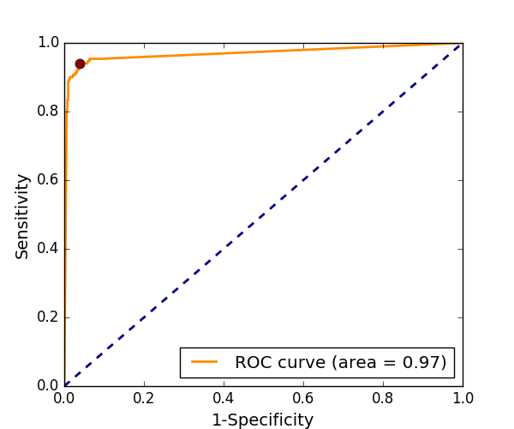
\includegraphics[width=0.49\textwidth + 0.49\marginparwidth + 0.49\marginparsep]{figures/paper-iii/Figure_4a.png}}
    \subfloat[]
    {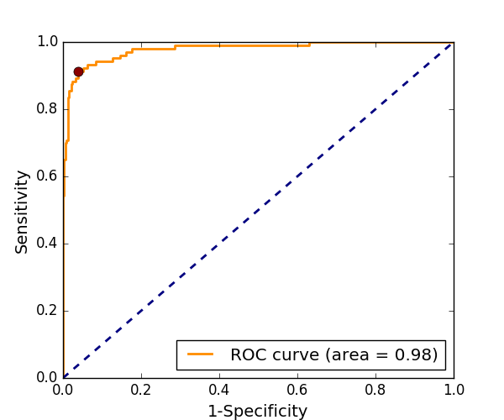
\includegraphics[width=0.49\textwidth + 0.49\marginparwidth + 0.49\marginparsep]{figures/paper-iii/Figure_4b.png}} \\
    \subfloat[]
    {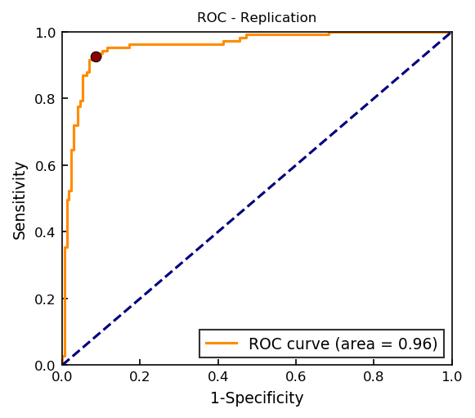
\includegraphics[width=0.49\textwidth + 0.49\marginparwidth + 0.49\marginparsep]{figures/paper-iii/Figure_4c.png}}
    \subfloat[]
    {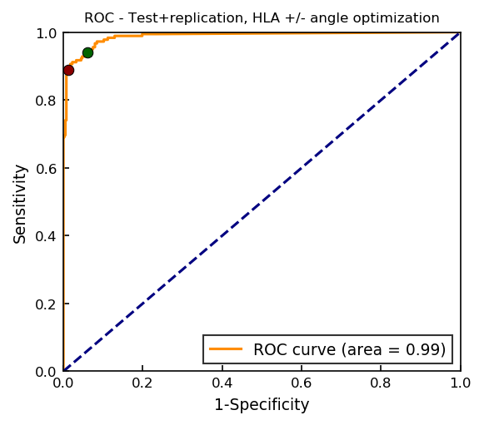
\includegraphics[width=0.49\textwidth + 0.49\marginparwidth + 0.49\marginparsep]{figures/paper-iii/Figure_4d.png}} \\
    \subfloat[]
    {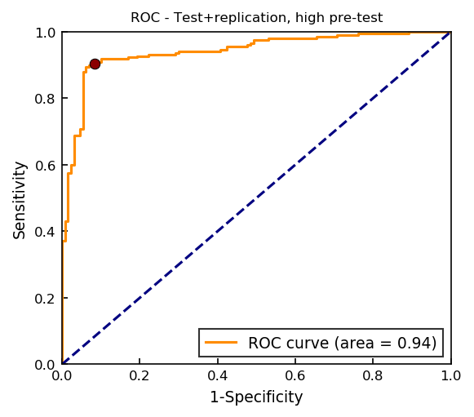
\includegraphics[width=0.49\textwidth + 0.49\marginparwidth + 0.49\marginparsep]{figures/paper-iii/Figure_4e.png}}
    \subfloat[]
    {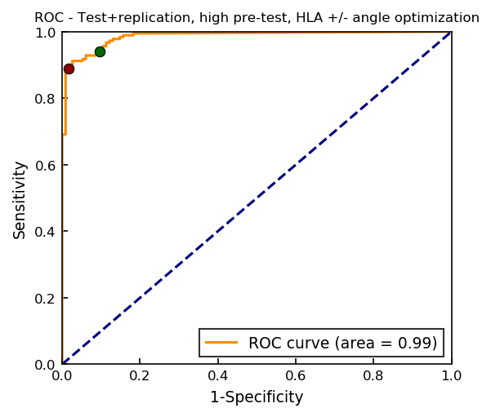
\includegraphics[width=0.49\textwidth + 0.49\marginparwidth + 0.49\marginparsep]{figures/paper-iii/Figure_4f.png}}
    \caption[Diagnostic receiver operating characteristics curves for narcolepsy model]{Diagnostic receiver operating characteristics curves for narcolepsy model displaying the trade-offs between sensitivity and specificity for the narcolepsy biomarker for (a) training sample, (b) testing sample, (c) replication sample, and (e) high pretest sample. 
    (d)–(f) Adding \ac{HLA} to model greatly increases specificity. 
    Cut-off thresholds are presented for models with (red dot) and without \ac{HLA} (green dot)}
    \label{fig:classification-sleep-disorders:paper-iii:figure-04}
    \end{adjustwidth*}
\end{figure}

To quantify narcolepsy-like behavior for a single recording, we generated features quantifying sleep stage dissociation using 16 sleep stage prediction models. 
These features were based on descriptive statistics and other features describing persistence of a set of new time series generated from every permutation product of the set of predicted sleep stages.

We also added features expected to predict narcolepsy based on prior work, such as \ac{REM} sleep latency and sleep stage sequencing parameters. 
A \ac{RFE} procedure was performed on extracted features with average outcome setting the optimal number of relevant features at 38~\cite{Guyon2002}. 

An optimal selection frequency cut-off of 0.40\graffito{That means including a feature if it was selected in \SI{40}{\percent} of the cross-validation runs} was determined using a cross-validation setup on the training data. 
The selected features are described in~\cref{tab:paperiii-supptable05} with detailed description of the eight most important features reported in~\cref{tab:paperiii-table04}.

Final predictions were achieved by creating a separate \ac{GP} narcolepsy classifier for each of the sleep scoring models used in the final implementation. 
The models were trained (tested) on data from seven (five) different cohorts with subsequent independent replication in two cohorts previously unseen by the algorithm, see~\cref{tab:classification-sleep-disorders:paper-iii:table-s01}.
The algorithm produced values between -1 and 1, with 1 indicating a high probability of \ac{NT1}.
A cut-off threshold of -0.03 was determined using cross-validation on the training dataset, which is shown with red dots in~\cref{fig:classification-sleep-disorders:paper-iii:figure-04}. 
This optimal trade-off achieves both high sensitivity and specificity, which is seen to translate well onto the test data and the replication sample in~\cref{fig:classification-sleep-disorders:paper-iii:figure-04}b-c.

In the training data, a sensitivity of \SI{94}{\percent} and specificity of
\SI{96}{\percent} was achieved, and in the testing data a sensitivity of \SI{91}{\percent} and specificity of \SI{96}{\percent} was achieved, while the sensitivity and specificity for the replication sample was \SIlist{93;91}{\percent}, respectively. 
When \ac{HLA} was added to this model (\cref{fig:classification-sleep-disorders:paper-iii:figure-04}d--f), the sensitivity changed to \SI{90}{\percent} and the specificity rose to \SI{99}{\percent}, and the cut-off threshold was updated to \num{-0.53} shown with green dots in~\cref{fig:classification-sleep-disorders:paper-iii:figure-04}d--f.
Furthermore, in the high pretest sample we obtained a sensitivity and specificity of \SIlist{90;92}{\percent}, which rose to \SIlist{90;98}{\percent} when adding \ac{HLA}.
More descriptive statistics including \SI{95}{\percent} confidence intervals are shown in~\cref{tab:paperiii-supptable06}.

\begin{table}
    % \centering
    \small
    \begin{adjustwidth*}{}{-\marginparwidth-\marginparsep}
    \begin{threeparttable}
    \caption[Description of most frequent features]{Eight most frequently selected features for \acs{NT1} detection.}
    \label{tab:paperiii-table04}
    % \begin{tabular*}{\textwidth+\marginparwidth+0.5\marginparsep}{@{}lcp{\textwidth}@{}}
    \begin{tabular}{@{}lcp{\marginparsep+\textwidth}@{}}
        \toprule
          & \textbf{Frequency} & \textbf{Description} \\
        \midrule
        1 & 1.00 & Time until \SI{5}{\percent} of the weighted sum of the product between \acs{W}, \acs{N2}, and \acs{REM} calculated at every epoch has accumulated. This feature expresses the known sleep stage dissociation and altered sleep timing.\\
        2 & 0.91 & Number of \acp{SOREMP} appearing throughout the recording.\\
        3 & 0.82 & Time until \SI{50}{\percent} of \ac{W} in recording has accumulated weighted by total amount of \ac{W}.\\
        4 & 0.82 & Shannon entropy of \ac{REM} sleep. This expresses the amount of information held in a signal, or in this case, how many different values the \ac{REM} sleep stage distribution obtains, \ie how consolidated phases of \ac{REM} are when the stage appears. \\
        5 & 0.68 & Maximum probability of \ac{W} obtained in a recording. \\
        6 & 0.68 & Maximum value obtained of the product between \ac{N2} and \ac{REM} probability in a recording.\\
        7 & 0.68 & Time until \SI{30}{\percent} of the epoch-by-epoch sum product between \ac{W} and \ac{N2} has accumulated, weighted by the sum total. \\
        8 & 0.64 & The time taken before \SI{10}{\percent} of the epoch-by-epoch sum product between \ac{W} and \ac{N1} has accumulated, weighted by the sum total.\\
        \bottomrule
    \end{tabular}
    \begin{tablenotes}
    \item %
    \describe{NT1}; %
    \describe{W}; %
    \describe{N1}; %
    \describe{N2}; %
    \describe{N3}; %
    \describe{REM}; %
    \describe{SOREMP}.
    \end{tablenotes}
    \end{threeparttable}
    \end{adjustwidth*}
\end{table}

\begin{table}
    % \centering
    \small
    \begin{adjustwidth*}{}{-\marginparwidth-\marginparsep}
    \begin{threeparttable}
    \caption[Narcolepsy biomarker performance]{Descriptive statistics on the evaluation of the narcolepsy biomarker in models with and without the \ac{HLA} biomarker. Mean value (top) and 95\% confidence interval (bottom).}
    \label{tab:paperiii-supptable06}
    \begin{tabular}{@{}llllllrr@{}}
        \toprule
        \textbf{Model}      & \textbf{Accuracy}, \% & \textbf{Sensitivity}, \% & \textbf{Specificity}, \% & \textbf{PPV}, \%  & \textbf{NPV}, \%  & \textbf{\acp{PSG}} & \textbf{\ac{NT1}}, \% \\ \midrule
        T                   & 0.95          & 0.91             & 0.96             & 0.88      & 0.97      & 444       & 0.24                       \\
                            & 0.92-0.97     & 0.84-0.96        & 0.93-0.98        & 0.80-0.93 & 0.95-0.99 &           &                            \\
        R                   & 0.92          & 0.93             & 0.91             & 0.87      & 0.95      & 321       & 0.28                       \\
                            & 0.88-0.95     & 0.87-0.97        & 0.87-0.95        & 0.80-0.93 & 0.92-0.98 &           &                            \\
        \multirow[t]{2}{0.175\textwidth}{T+R, HLA} & 0.96          & 0.9              & 0.99             & 0.97      & 0.95      & 584       & 0.31                       \\
                            & 0.94-0.97     & 0.84-0.93        & 0.98-1.00        & 0.94-0.99 & 0.93-0.97 &           &                            \\
        \multirow[t]{2}{0.175\textwidth}{T+R, HLA, optim.}    & 0.94          & 0.94             & 0.94             & 0.88      & 0.97      & 584       & 0.31                       \\
                            & 0.92-0.96     & 0.90-0.97        & 0.92-0.96        & 0.83-0.92 & 0.95-0.99 &           &                            \\
        \multirow[t]{2}{0.175\textwidth}{HPT, no HLA.}        & 0.91          & 0.9              & 0.92             & 0.94      & 0.86      & 335       & 0.61                       \\
                            & 0.87-0.94     & 0.86-0.94        & 0.86-0.96        & 0.91-0.97 & 0.80-0.91 &           &                            \\
        \multirow[t]{2}{0.175\textwidth}{HPT, HLA}            & 0.93          & 0.9              & 0.98             & 0.99      & 0.85      & 296       & 0.61                       \\
                            & 0.90-0.95     & 0.84-0.93        & 0.96-1.00        & 0.97-1.00 & 0.79-0.91 &           &                            \\
        \multirow[t]{2}{0.175\textwidth}{HPT, HLA, optim.}    & 0.93          & 0.94             & 0.9              & 0.94      & 0.9       & 296       & 0.61                       \\
                            & 0.90-0.95     & 0.90-0.97        & 0.85-0.95        & 0.90-0.97 & 0.85-0.95 &           &                            \\ \bottomrule
    \end{tabular}
    \begin{tablenotes}
    \small 
    \item Performance on models with \ac{HLA} typing is reported for both regular and optimized threshold, since the \acs{ROC} curve changes by adding \ac{HLA}. %
    \describe{HLA}; %
    \describe{ROC}; %
    \describe{NT1}; %
    T, test dataset; %
    R, replication dataset; %
    HPT, high pre-test probability dataset; %
    PPV, positive predictive value (precision); %
    NPV, negative predictive value.
    \end{tablenotes}
    \end{threeparttable}
    \end{adjustwidth*}
\end{table}

\subsection{Discussion}

Using our models, and considering how typical \ac{NT1} behaved in our sleep stage machine learning routines, we extracted features that could be useful to diagnose this condition.
% \Ac{NT1} is characterized by a loss of hypocretin-producing cells in the hypothalamus and can be best diagnosed by measuring hypocretin levels in the \ac{CSF}~\cite{Peyron2000,Mignot2002}, a procedure that requires a lumbar puncture, which is rarely performed in the United States\todo{Need sources on this and in Europe}.
% At the symptomatic level, \ac{NT1} is characterized by sleepiness, cataplexy\graffito{cataplexic episodes are defined by muscle weakness during wakefulness often triggered by strong emotions.} and numerous symptoms reflecting poor nocturnal sleep (insomnia) and symptoms of \textit{dissociated REM sleep}.
% Dissociated \ac{REM} sleep is reflected in the hypnogram/hypnodensity by the presence of unusual states of consciousness where \ac{REM} sleep intermingles with wakefulness thus producing disturbing reports of dreams that interrupt wakefulness and seem real\graffito{this is also called hypnagogic halluciations.}, or episodes where the sleeper is awake, but paralyzed, as in normal REM sleep\graffito{this is also called sleep paralysis.}.
% The current gold standard for \ac{NT1} diagnosis is the presence of cataplexy and a positive \ac{MSLT}.
% In a recent large study of the \ac{MSLT}, specificity and sensitivity for \ac{NT1} was \SIlist{98.6;92.9}{\percent} in comparing \ac{NT1} versus controls, and \SIlist{71.2;93.4}{\percent} in comparing \ac{NT1} versus other hypersomnia cases~\cite{Andlauer2013}.

\Cref{tab:paperiii-table04,tab:paperiii-supptable05} reveal features found in nocturnal \acp{PSG}s that discriminate \ac{NT1} from non-narcolepsy. 
One of the most prominent features, short latency \ac{REM} sleep, bears great resemblance to the \ac{REM} sleep latency, which is currently used clinically to diagnose narcolepsy. As short \ac{REML} is calculated using fuzzy logic, it represents a latency where accumulated sleep suggests high probability of \ac{REM} sleep occurrence\graffito{As opposed to a discrete \ac{REM} latency scored by a technician}. 
A short \ac{REM} latency during \ac{PSG} recording\graffito{Short in this case typically means less than \SI{15}{\minute}} is extremely specific (\SI{99}{\percent}) and moderately sensitive (\SIrange{40}{50}{\percent}) for \ac{NT1} classification~\cite{Andlauer2013,Reiter2015}. 
The remaining selected features also describe a generally altered sleep architecture, particularly between \ac{REM} sleep, light sleep\graffito{Here light sleep is comprised of \ac{N1} and \ac{N2}} and \ac{W}.
These dissociations mirror aspects of narcolepsy which are already known and thus reinforce their validity as biomarkers.

For example, the primary feature, as determined by the \ac{RFE} algorithm, was the time it took to reach\SI{5}{\percent} of the accumulated sum of the probability products between stages \ac{W}, \ac{N2} and \ac{REM}, which reflects the uncertainty between \ac{W}, \ac{REM} and \ac{N2} sleep at the beginning of the night. 
Specifically, for the \textit{n}th epoch, the model will output probabilities for each sleep stage, and the proto-feature \( \boldsymbol{\Phi}_n \) is calculated as
\begin{equation}
    \boldsymbol{\Phi}_n = \func{p}{\wake} \times \func{p}{\nII} + \func{p}{\wake} \times \func{p}{\rem} + \func{p}{\nII} \times \func{p}{\rem}
\end{equation}
The feature value is then calculated as the time it takes in minutes for the accumulated sum of \( \boldsymbol{\Phi}_n \) to reach \SI{5}{\percent} of the total sum \( \sum_n \boldsymbol{\Phi}_n \). 
Since each probability product in \( \boldsymbol{\Phi}_n \) reflects the staging uncertainty between each sleep stage pair, \( \boldsymbol{\Phi}_n \) alone reflects the general sleep stage uncertainty for that specific epoch as predicted by the model. 
A high feature value is attained for epoch \textit{n} when \ac{N2}, \ac{W} and \ac{REM} are of equal probability and the remaining two sleep stages are close to zero. 
A \ac{PSG} with a high staging uncertainty between sleep and wake early in the night would reach the \SI{5}{\percent} threshold rapidly.

Using these features, we determined an optimal cut-off that discriminated narcolepsy from controls and other patients with specificity and sensitivity as high as the \ac{MSLT}\graffito{See also~\cref{tab:paperiii-supptable06} for details}, notably when \ac{HLA} typing is added. 
This is true for both the test and replication samples. 
Although we observed a small drop in specificity in the replication sample, the performance was similar to the \ac{MSLT} when the efficacy of the detector was tested in the context of naive patients with hypersomnia in the high pretest probability sample.

Furthermore, \acp{MSLT} requires that patients spend an entire night and day in a sleep laboratory. 
This novel biomarker could allow for improved recognition of ac{NT1} cases at a reduced cost by only requiring a standard \ac{PSG} screening as used for other sleep pathologies, such as \ac{OSA}.
A positive predictive value could also be provided depending on the nature of the sample and known narcolepsy prevalence\graffito{This prevalence is low in general population screening, intermediary in a overall clinic population sample, and high in hypersomnia cohorts}.
It also opens the possibility of using home sleep recordings for diagnosing narcolepsy. 
In this direction, because of the probabilistic and automatic nature of our biomarker, estimates from more than one night could be automatically analyzed and combined over time ensuring improved prediction. 
However, it is important to note that this algorithm will not replace the \ac{MSLT} in the ability to predict excessive daytime sleepiness through the measure of mean sleep latency across daytime naps, which is an important characteristic of other hypersomnias.

When the staging data were presented as hypnodensity distributions, the model conveyed more information about the subject than through a hypnogram alone.
This led to the creation of a biomarker for narcolepsy that achieved similar performance to the current clinical gold standard, the MSLT, but only requires a single sleep study.
If increased specificity is needed, for example, in large-scale screening, HLA or additional genetic typing brings specificity above 99\% without loss of sensitivity.
This presents an option for robust, consistent, inexpensive and simpler diagnosis of subjects who may have narcolepsy, as such tests may also be carried out in a home environment.

This study shows how hypnodensity graphs can be created automatically from raw sleep study data, and how the resulting interpretable features can be used to generate a diagnosis probability for \ac{NT1}.
Another approach would be to classify narcolepsy directly from the neural network by optimizing the performance not only for sleep staging, but also for direct diagnosis by adding an additional softmax output, thereby creating a multitask classifier.
This approach could lead to better predictions, since features are not then limited to by a designer imagination. 
A drawback of this approach is that features would no longer be as interpretable and meaningful to clinicians. 
If meaning could be extracted from these neural network generated features, this might open the door to a single universal sleep analysis model, covering multiple diseases.
Development of such a model would require adding more subjects with narcolepsy and other conditions to the pool of training data.
